\documentclass[10pt, compress]{beamer}

\usetheme{m}

\usepackage{booktabs}
\usepackage[scale=2]{ccicons}
\usepackage{minted}

\usepgfplotslibrary{dateplot}

\usemintedstyle{trac}

\title{Betti Numbers and Alpha Complexes}

\begin{document}

\maketitle

\begin{frame}[fragile]
    \frametitle{Toplogical spaces}
    A topological space may be defined as a set of points, along with a set of
    neighbourhoods for each point, that satisfy a set of axioms relating points
    and neighbourhoods.
    \begin{figure}
        \centering
        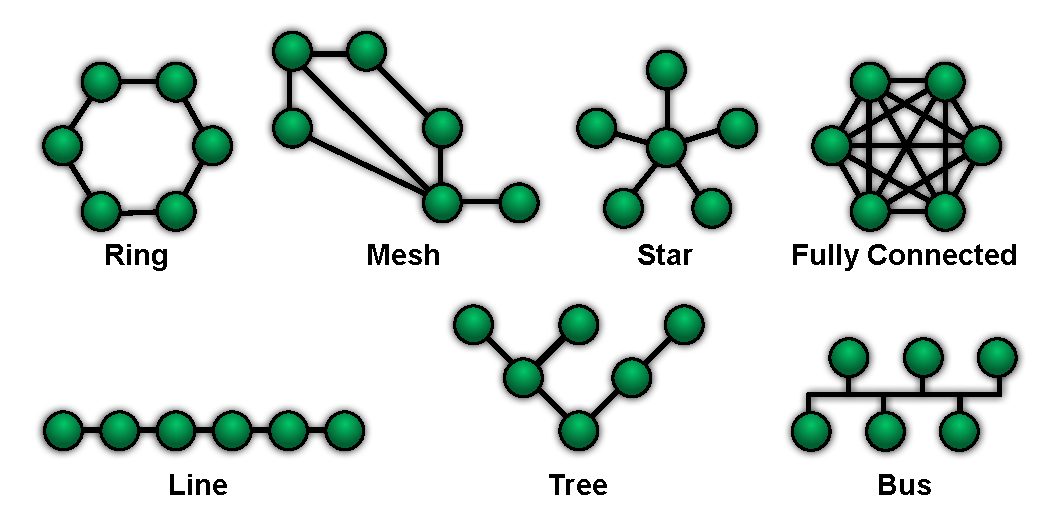
\includegraphics[width=0.8\textwidth]{fig/topologies.pdf}
    \end{figure}
\end{frame}
\begin{frame}[fragile]
    \frametitle{Betti numbers}
    Betti numbers are used to distinguish topological spaces based on the
    connectivity of n-dimensional simplicial complexes.
    The k'th Betti number refers to the number of k-dimensional holes on a
    topological surface.
    \begin{itemize}
        \item $b_0$ is the number of connected components
        \item $b_1$ is the number of one-dimensional or "circular" holes
        \item $b_2$ is the number of two-dimensional "voids" or "cavities"
    \end{itemize}
\end{frame}
\begin{frame}[fragile]
    \frametitle{Betti numbers by example}
    Examples of Betti numbers for a complex.
    \begin{figure}
        \centering
        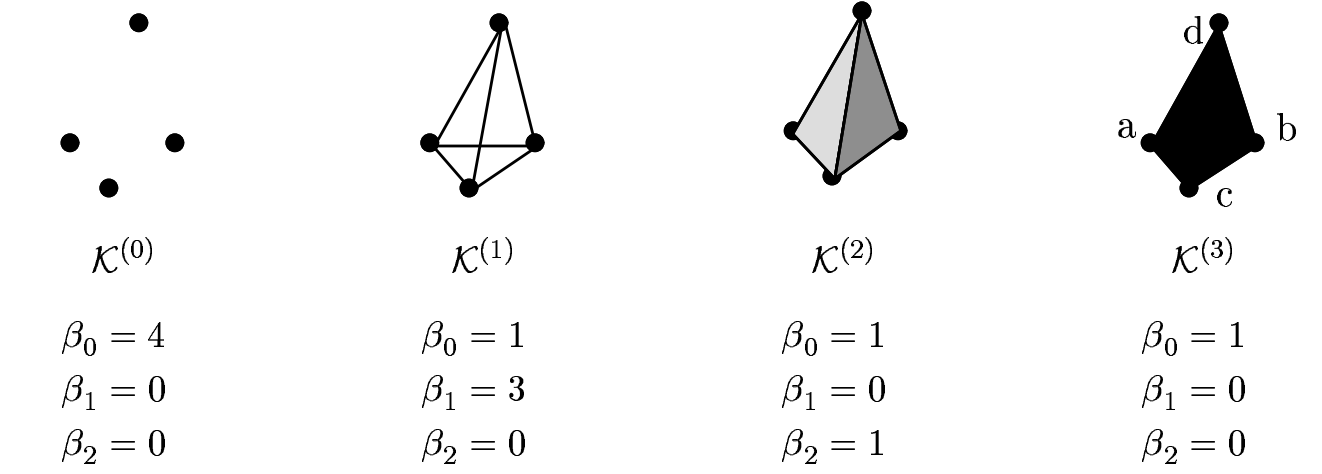
\includegraphics[width=1.0\textwidth]{fig/betti_example.png}
    \end{figure}
\end{frame}

%\begin{frame}[fragile]
%    \frametitle{Simplices}
%    A simplex (plural simplexes or simplices) is a generalization of the
%    notion of a triangle or tetrahedron to arbitrary dimensions.
%    \begin{figure}
%        \centering
%        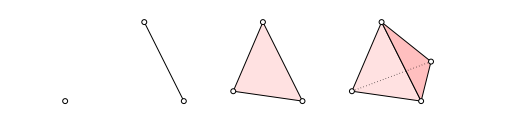
\includegraphics[width=0.56\textwidth]{fig/simplices.png}
%    \end{figure}
%    In topology and combinatorics, it is common to “glue together” simplices
%    to form a simplicial complex.
%\end{frame}

\section{An algorithm for Betti numbers}
\begin{frame}[fragile]
    \frametitle{Filtering a complex by simplices}
    Incremental algorithm, that uses filtration.
    \begin{figure}
        \centering
        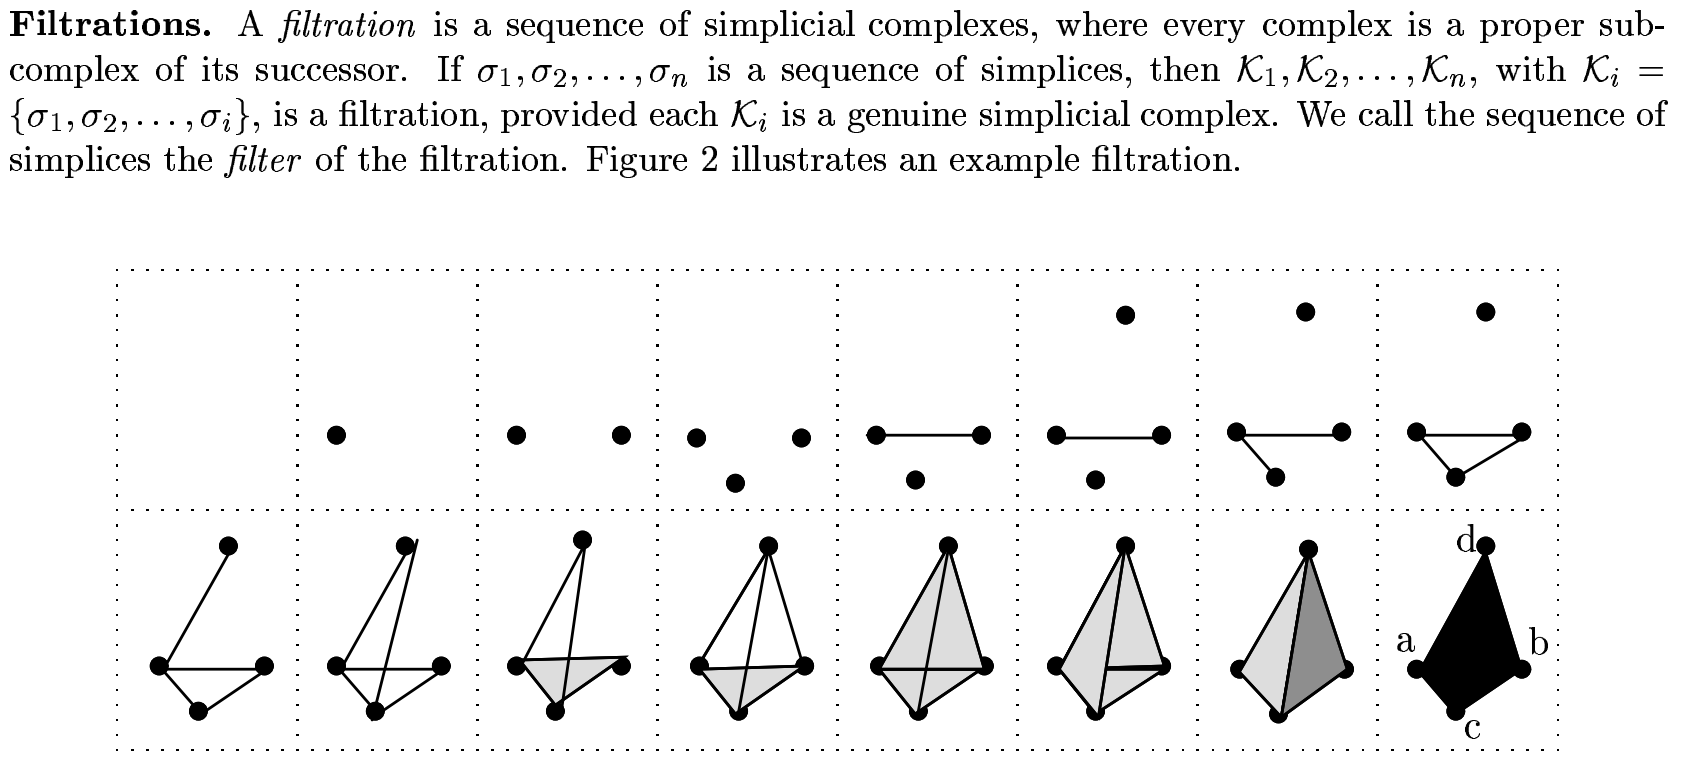
\includegraphics[width=1.0\textwidth]{fig/filtering.png}
    \end{figure}
\end{frame}
\begin{frame}[fragile]
    \frametitle{The algorithm}
    The incremental algorithm:
    \begin{figure}
        \centering
        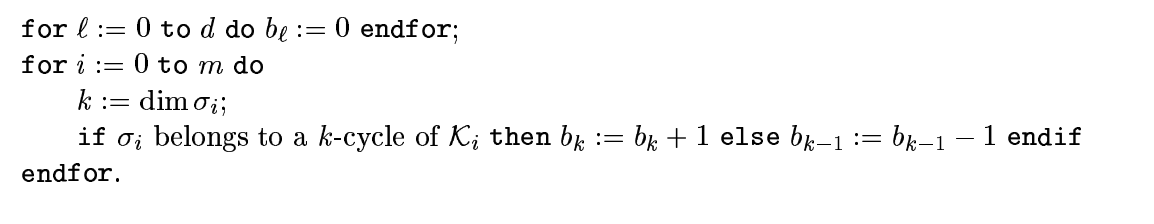
\includegraphics[width=1.0\textwidth]{fig/betti_algo.png}
    \end{figure}
    Lets do a small example.
\end{frame}
\begin{frame}[fragile]
    \frametitle{Running time}
    In practice cycles are checked by using sets.\\
    Running time is $O(\alpha(n)n)$, where $\alpha(n)$ is the inverse
    ackermann function. and $n$ is the sum of $k$-simplices.
\end{frame}

\section{Alpha complexes}
\begin{frame}{Alpha complexes}
    Definition goes here.
\end{frame}
\section{Persistence and simplification}
\begin{frame}{Simplification}
    explain
    \begin{figure}
        \centering
        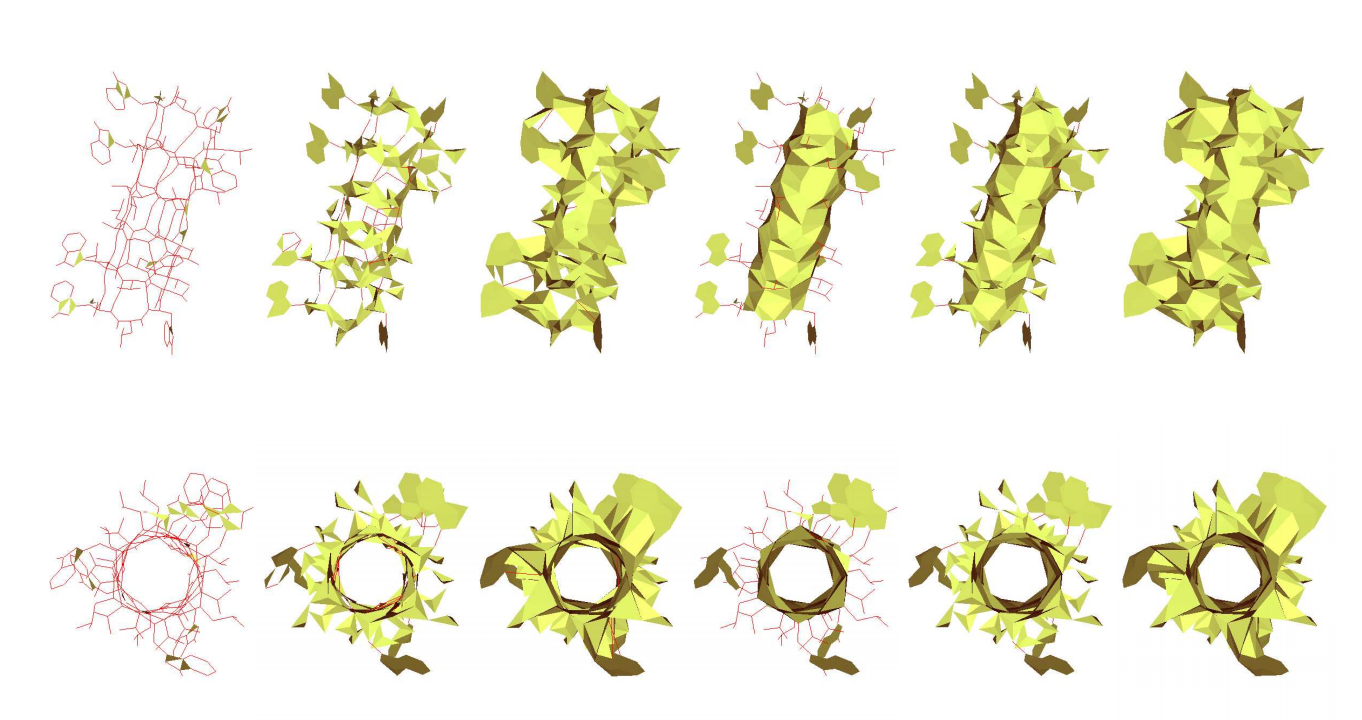
\includegraphics[width=0.8\textwidth]{fig/simplification.png}
    \end{figure}
\end{frame}
\begin{frame}{Filter}
    explain
    \begin{figure}
        \centering
        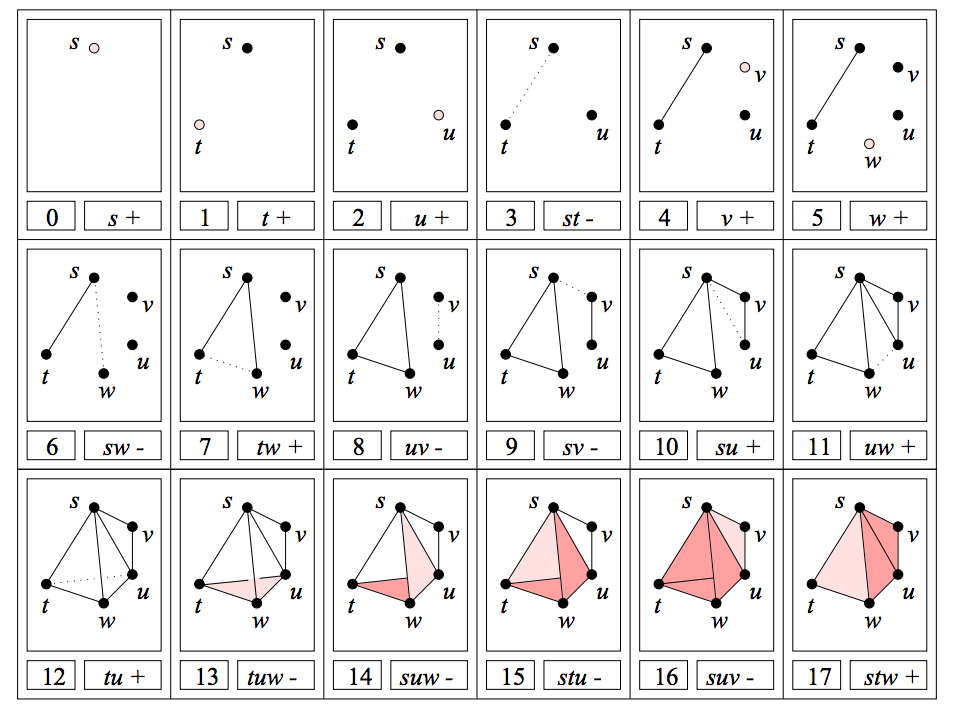
\includegraphics[width=0.8\textwidth]{fig/filter.png}
    \end{figure}
\end{frame}
\begin{frame}{Pair datastructure}
    explain
    \begin{figure}
        \centering
        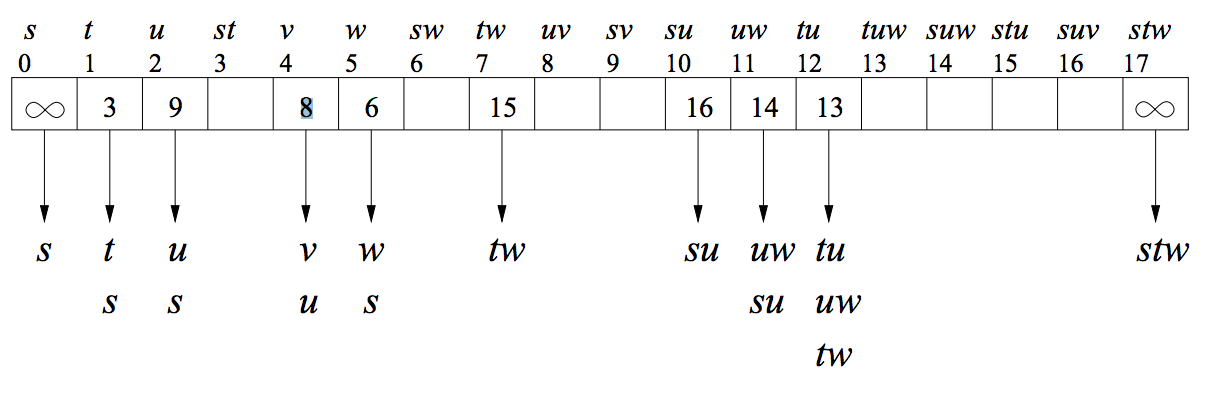
\includegraphics[width=0.8\textwidth]{fig/pairs.png}
    \end{figure}
\end{frame}

\begin{frame}{Pairs persistence}
    explain
    \begin{figure}
        \centering
        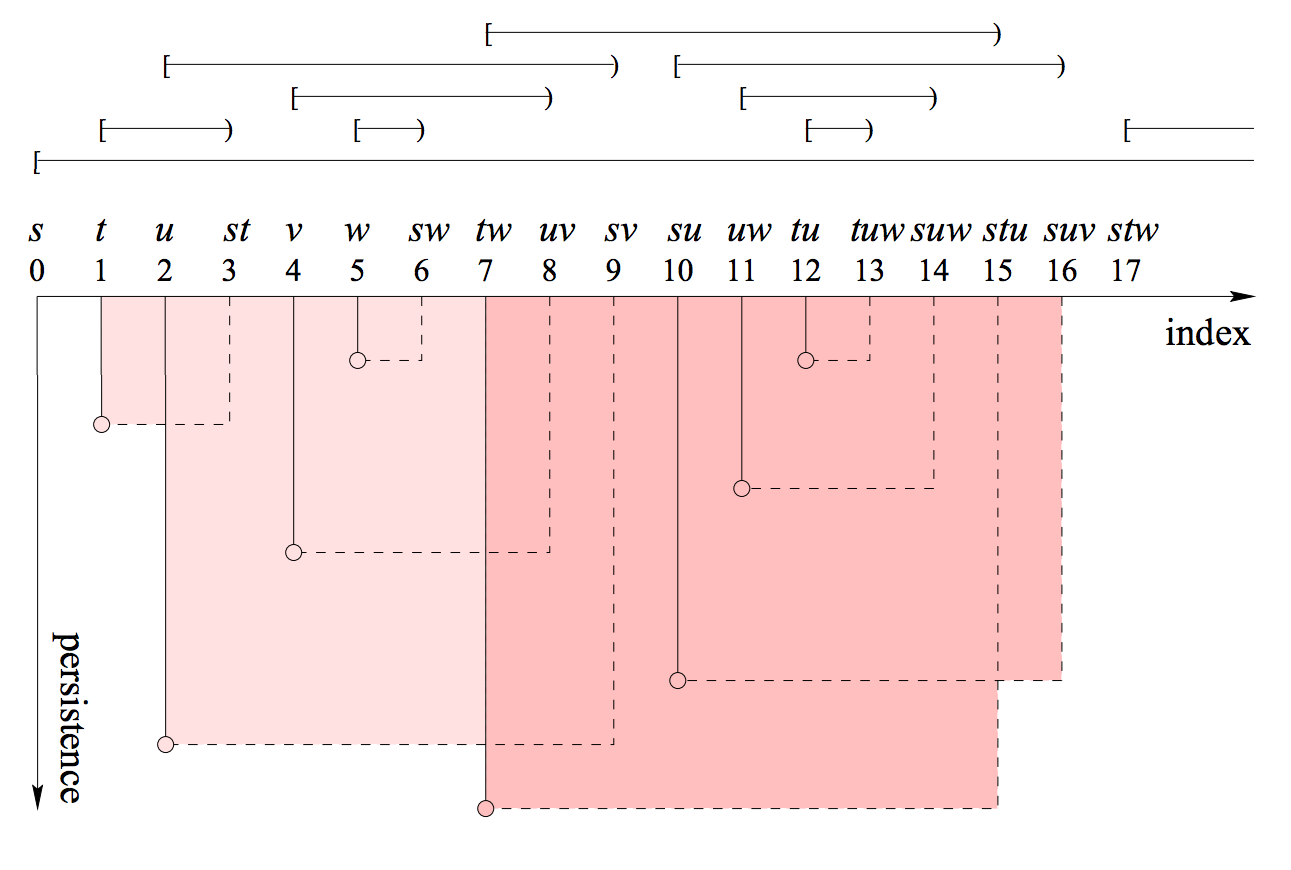
\includegraphics[width=0.8\textwidth]{fig/pair_sim.png}
    \end{figure}
\end{frame}


\end{document}
